\scanpage{223}
% archive sheet number: 222

Il suffirait de construire $X$ projectif lisse sur $k$, tel que $H^{\unsure{*|\alpha}}(X_{\unsure{w|v}},\mathbb{Z})$ et $H^*(X_{\unsure{v|w|v'}},\mathbb{Z})$ non isomorphes comme \uline{anneaux}.

% slanted
\margin{Peut-on remplacer $\mathbb{Z}$ par $\mathbb{R}$ ??}

On devrait mettre Serre à contribution.

\figure{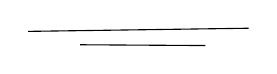
\begin{tikzpicture}[x=1cm,y=1cm]\draw (0,.17)--(2.8,.21); \draw (.66,0)--(2.25,-.01);\end{tikzpicture}}

Soit $k$ un corps de nbs, $v_0$ une place de $k$, $M$ un motif sur $k$, d'où $G_{M v_0}=G_{v_0}$ groupe algébrique \uline{défini sur} $\mathbb{Z}$. Toute autre place \deleted{\unsure{$w$}} $v$ définit un fibré principal homogène $P_v$ sous $G_{v_0}$, \unsure{et} si on admet ce qui a été \deleted{dit} \inserted{conjecturé} plus haut, \inserted{si $M$ est pris assez grand,} $v\ne v'\Longrightarrow P_v\not\simeq P_{v'}$. On peut aller plus loin et se demander si \deleted{\unsure{tout}} (pour $M$ assez grand) \uline{$\forall$} fibré principal homogène $P$ sous $G_{v_0}$ provient d'une place $v$ \deleted{\unsure{calculer|réelle}} / \deleted{\unsure{les}} On \deleted{a} peut poser

% slanted
\margin{/ Attention, la condition d'avoir un isomorphisme de foncteurs $\unsure{\zeta|\xi}(M)\otimes_{\mathbb{Z}}\mathbb{C}\simeq M_\infty\otimes_k\mathbb{C}$, satisfaisant aux conditions de compatibilité genre Riemann-Hodge, risque d'être une condition restrictive sérieuse\unsure{....|...}}

\[
G_{Mv_{\unsure{2|0|\alpha}}}(\mathbb{Z})=\unsure{\Pi|\pi}^{1}_{M}(k,v) :
\]

ces groupes à priori ne sont pas isomorphes : groupes \uline{fondamentaux \inserted{(arithmétiques)} discrets}.
